\documentclass{../../text-style}

\texttitle{Лекция 12: Непрерывное развёртывание}

\begin{document}

\maketitle
\thispagestyle{empty}

\attribution{Тимофей Александрович Брыксин, бывш. доцент кафедры системного программирования СПбГУ}

Представьте, что к вам приходит начальник, и просит продемонстрировать последнюю версию проекта заказчику. У вас десяток разработчиков, каждый из которых работает над собственной фичей (возможно даже в собственной ветке), но никто из них не имеет версии, в которой содержится вся функциональность в стабильном виде. То есть у вас есть код, он компилируется, даже модульные тесты проходят (может быть даже на интеграционном сервере), но выкатить новую работоспособную версию так же быстро, как скомпилировать код, вы не можете.

Другая задача: в вашей системе найден критический баг, компания теряет кучу денег с каждым часом. Вы знаете, как её исправить: требуется изменение в одной строчке кода в библиотеке, используемой практически всеми компонентами системы. Опять же задача~--- быстро собрать и выкатить версию в production-окружение, и часто опять же эта задача занимает слишком много времени, если о ней никто не подумал заранее.

Развёртывание приложений многими программистами считается не особо важным делом (ну конечно, это же не написание кода!), и поэтому ему не уделяется достаточно времени и сил. В итоге <<сэкономленное>> время приходится тратить раз за разом с каждым новым релизом. Во многих проектах цикл развёртывания новой версии может измеряться неделями или даже месяцами, а процесс не определён и, как следствие, не повторяем. Он проводится вручную и часто требует работы специально подобранной команды, даже для развёртывания локально в рамках компании. 

Такой долгий цикл релизов был вполне допустим в 90-е годы, когда ПО выпускали на дисках, и чаще, чем раз в год, клиенты не готовы были покупать новую версию. Современные компании релизят свои веб-продукты по нескольку раз за день. И это могут быть весьма большие проекты с обширной кодовой базой. По аналогии со сборкой проекта развёртывание приложений должно быть быстрым и повторяемым процессом. Если их решение занимает слишком много времени, то это повод задуматься. Вот некоторые важные вопросы, на которые стоит ответить каждому проекту: 

\begin{itemize}
    \item Как быстро изменения в 1 строчку кода попадают к пользователям?
    \item Сколько для этого требуется усилий?
    \item Насколько это процесс повторяем?
    \item Сколько человек должно быть вовлечено в этот процесс?
\end{itemize}

Было бы ошибкой думать, что проблемы с развёртыванием решатся с выпуском первой версии: первый раз как-нибудь зарелизим, а потом будем просто повторять по накатанной. Учитывая, что для успешных продуктов сопровождение является самой длительной стадией жизненного цикла, преобладающая часть стоимости процесса развёртывания ПО приходится на период времени именно после первого релиза: это добавление новых фич и исправление дефектов, причём зачастую условия и окружение для развёртывания тоже меняются. Всё это особенно актуально, если разработка носит итеративный характер, где функциональность поставляется пользователям частями. Практика непрерывного развёртывания (Continuous Delivery) основывается на этих идеях и позволяет сократить время и риски, связанные с развёртыванием новых версий, за счёт автоматизации процесса, упрощения взаимодействий между членами команды, автоматического тестирования, учащения релизов и прочих практик, про которые мы будем говорить в этой лекции.

Некоторые думают, что инфраструктуру для развёртывания имеет смысл строить только для больших проектов. Однако проекты имеют тенденцию разрастаться, и часто довольно быстро, да и решения, которые вы принимаете в самом начале проекта, имеют большой эффект на то, как он будет эволюционировать в дальнейшем, какова культура разработки будет у его команды.

\section{Некоторые антипаттерны управления релизами}

Как уже отмечалось выше, во многих проектах выпуск новых версий весьма утомителен. Окружения, в которые помещаются эти версии, часто настраиваются индивидуально под каждую версию: устанавливается third-party ПО, копируются сами артефакты разворачиваемого ПО, копируется и донастраивается через администраторские консоли конфигурационная информация, копируются данные для собственно работы ПО, а затем всё запускается (в случае распределённых систем, программа за программой).

В этом процессе очень многое может пойти не так: если какой-то шаг не будет идеально выполнен, ПО может не запуститься корректно. И далеко не сразу может быть понятно, что пошло не так и на каком шаге.

\subsection{Антипаттерн 1: ручное развёртывание}

Многие компании выполняют описанный выше процесс развёртывания вручную. Каждый шаг процесса рассматривается как отдельный и атомарный, выполняемый отдельным человеком или даже командой. Это приводит к возможности человеческой ошибки, связанной с невнимательностью, незнанием, разницей в порядке или времени выполнения этих шагов.

Основным признаком данного антипаттерна часто является подробная документация, описывающая процесс развёртывания, включая то, что может пойти не так. Поддержка актуальности подобной документации~--- весьма трудоёмкий процесс, да и мы все знаем, как сильно программисты любят писать и поддерживать актуальную документацию. Самое плохое, если документация перестаёт быть актуальной, а все знания сосредотачиваются в голове одного или нескольких экспертов (и тут начинает играть свою роль bus factor). И при всём этом процесс развёртывания редко можно назвать очень увлекательным (особенно учитывая, что критерием завершения процесса часто является ручная проверка работоспособности приложения), так что эти эксперты тратят своё высокооплачиваемое время не самым эффективным образом.

Для первых версий подобный ручной процесс может быть необходимостью, однако далее он должен быть автоматизирован. От человека должно требоваться всего два действия: выбрать нужную версию и нажать кнопку <<Deploy>>. Всё остальное должно осуществляться автоматически.

Отлаженные один раз скрипты больше не ошибаются. Они сами являются и инструментом развёртывания, и документацией к этому процессу. Скрипты детерминированы и не склонны к спонтанным ошибкам. Скрипт должен написать и отладить эксперт, но запустить его под силу человеку любой квалификации.

\sout{Слава роботам!} Автоматизация~--- друг человека.

\subsection{Антипаттерн 2: развёртывание только после завершения разработки}

В этом сценарии первый раз ПО попадает в production-like окружение (например, в рамках песочницы внутри компании), когда разработка уже закончена (что бы под этим ни понимали разработчики). Если тестировщики и привлекались к работе до этого момента, они тестировали всё это на своих компьютерах или в специальном окружении. Люди, ответственные за процесс развёртывания, в этот момент могут видеть ПО в первый раз (особенно если в компании за этот процесс отвечает отдельная команда). А разработчики могут иметь своё, очень особое мнение о том, каким будет production-окружение для их софта.

Подобная ситуация может складываться не обязательно из-за раздолбайства или непредусмотрительности разработчиков или менеджеров. Иногда окружение приложения крайне затратно для воспроизведения локально (например, если вы делаете систему пожаротушения для нефтяной вышки, построить копию вышки у себя в офисе для тестирования вы вряд ли сможете), либо есть какие-то другие ограничения (уникальность, безопасность и т.п.).

В таких случаях разработчики могут просто физически не иметь доступа к production-окружению, они собирают инсталляторы, конфигурационные файлы, схемы баз данных, документацию и т.п. и передают их людям, которые будут отвечать за размещение всего этого. Коммуникации между этими двумя командами в силу разных причин не всегда могут быть хорошо выстроены. Например, команды могут быть разделены территориально, находиться в разных компаниях или вообще не знать ничего друг о друге. Обратная связь до разработчиков, разумеется, в таких случаях в желаемом объёме не доходит. Но и команде развёртывания в такой ситуации при возникновении вопросов скорее приходится угадывать замысел разработчиков, а то делать какие-то изменения в коде или окружении целевого ПО. При этом если подобные догадки оказываются неверными, функционирование системы может быть нарушено или затруднено. Но даже если предположения оказываются верными и изменения сделаны по делу, они всё равно не попадут к разработчикам и в последующих версиях их нужно будет накатывать заново. Такая ситуация явно не способствует улучшению качества системы.

Если же обе эти команды находятся в рамках одной компании и имеют способы взаимодействовать друг с другом, каналы коммуникаций и политика взаимодействия между отделами тоже могут быть самыми разными. При должном уровне бюрократии коммуникации легко превращаются в ticketing hell, когда всё общение идёт только через систему управления задачами или широковещательные рассылки в электронной почте.

Выход вполне очевиден~--- максимально интегрировать процесс тестирования, размещения и выпуска ПО в процесс разработки. Таким образом, когда придёт время выпускать в мир новую версию, этот процесс уже не будет казаться таким страшным и рисковым. Это может потребовать дополнительных как организационных, так и технических расходов, однако даст вам уверенность в том, что когда придёт время, всё будет идти, как положено.

\subsection{Антипаттерн 3: ручное управление окружением в продакшене}

Когда управление конфигурацией продакшен-окружения выполняется вручную, все изменения часто делаются <<на горячую>> прямо на самих серверах. Например, это может быть изменение строки подключения к СУБД или размер пула потоков. В большинстве случаев это приводит к тому, что о сделанных изменениях знают только те, кто их внесли, и эта информация не попадает обратно к разработчикам. А ведь это может быть весьма критичная информация, которая не позволит в следующий раз развернуть ПО как положено. Последствиями такого неаккуратного управления окружением становится то, что процесс развёртывания не является повторяемым, становится крайне сложно откатиться к предыдущей развёрнутой стабильной версии, разные узлы вычислительной сети настроены и работают по-разному, и т.д. В крайних случаях может даже доходить до того, что вообще никто не имеет представления о том, какая именно версия ПО, базы данных или третьестороннего ПО сейчас крутится на боевом сервере.

\section{Частые автоматизированные релизы}

Чем быстрее мы можем выкатить релиз, тем быстрее мы проверим правильность и адекватность внесённых изменений и исправлений, тем быстрее это ПО сможет приносить пользу и доход. Но при этом, разумеется, ПО должно быть должного качества, иначе им просто никто не будет пользоваться. Итого, цель~--- научиться выпускать высококачественный полезный софт, причём делать это быстро, эффективно и надёжно. Хорошим инструментом для достижения этой цели являются частые автоматизированные релизы. 

\begin{itemize}
    \item Если процесс сборки, тестирования и развёртывания не автоматизирован, он не является надёжным и повторяемым (см. антипаттерн 1). А значит, ни о каком достойном уровне качества с гарантией говорить не приходится.
    \item Если релизы частые, то и дельта между ними будет не сильно большая. Это существенно снижает риски выкатывания некорректного нового релиза и необходимости отката к прошлой версии. Небольшие релизы поощряют (а часто и требуют) быструю обратную связь: быстро узнаём о проблемах, быстро на них реагируем.
\end{itemize}

Автоматизированная обратная связь важна также и в рамках самого процесса разработки. Большая часть ПО может быть разделена на четыре составляющих: исполняемый код, его конфигурация, окружение и данные. Если меняется какая-то из этих составляющих, это влияет на работу и всей системы в целом. (А это, как минимум, значит, что всё это нужно где-то хранить и следить за вносимыми изменениями.) Каждое изменение в артефакты проекта должно мгновенно генерировать какую-либо обратную связь: смена статуса в системе мониторинга, электронное письмо разработчикам или что-то ещё. Подобная скорость реагирования невозможна, если, например, за сборку проекта отвечает особый человек или всё тестирование проводится вручную.

Когда процессы автоматизированы, единственный оставшийся параметр~--- объём вычислительных ресурсов, который вы выделяете на задачу. Много тестов и они долго выполняются~--- запустите тесты параллельно на большем количестве серверов. И стоить это будет меньше, чем нанять дополнительного человека на эту работу. Да и люди, которые раньше выполняли рутинную и скучную работу, теперь могут заняться чем-то более интересным. Уж не говоря о снижении общего уровня стресса, который ассоциируется у людей с выкатыванием в production новый версий в ручном режиме. Когда любая ошибка может повлечь за собой потерю денег или репутации компании. Когда код, который работал локально, отказывает работать на целевом сервере, и требуется отладка и внесение изменений прямо <<по живому>>, часто под давлением руководства или заказчика. И совершенно другие ощущения разработчик испытывает, когда выкатывание новой версии занимает несколько минут или секунд, происходит нажатием одной кнопки, и если что-то пошло не так, может быть отменено в течение тех же минут или секунд.

Кроме того, внедрение подобного инструмента может дать членам команды дополнительные возможности, крайне полезные в их деятельности. Например, тестировщик теперь может в несколько кликов развернуть у себя на машине или в контролируемом окружении любую из прошлых версий ПО и сравнить её поведение с поведением текущей версии. Члены группы поддержки могут тем самым воспроизвести ошибки, проявляющейся у пользователей в продакшене, а также заменить развёрнутую там последнюю версию на одну из прошлых и более стабильных. Разработчики нажатием одной кнопки могут убедиться, что внесённые ими изменения не ломают процесс сборки и работы системы, и эти изменения готовы к публикации. Автоматизация сложных и рутинных процессов позволяет людям работать продуктивнее и производить продукт более высокого качества в более краткие сроки.

Ещё один аспект, с которым может помочь внедрение частых автоматизированных релизов~--- снижение количества ошибок в выпускаемом ПО. И в первую очередь это ошибки, связанные с развёртыванием. Правильные версии всех компонент, схем баз данных, конфигурации серверов и приложений и т.д. Со всеми этими ошибками весьма эффективно помогает бороться конфигурационное управление. Сейчас уже никого не удивишь использованием систем контроля версий, однако версионируя конфигурационные файлы, скрипты создания БД, скрипты сборки и тестирования, конфигурационные файлы сторонних приложений или даже операционной системы и т.п., мы убеждаемся, что наш код будет работать именно в том окружении, в котором мы предполагаем. Все эти настройки окружения играют не меньшую роль, чем логика, реализованная в самом приложении, а изменить их часто гораздо проще: изменение в коде чтобы вступить в силу требует как минимум перекомпиляции приложения со всеми синтаксическими проверками, прогоном тестов и т.п., а простая опечатка в конфигурационном файле может пройти практически незаметно. Хранение всех настроек окружения в системе контроля версий с последующим автоматическим получением их скриптами сборки и развёртывания позволяет убрать человеческий фактор, повышая надёжность всего процесса в целом.

\section{Принципы непрерывного развёртывания}

Идеи, описанные далее, составляют основу движения Continuous Delivery. Как и многие другие практики Agile, они появились как обобщение удачных практик из реальных проектов и вместе составляют основу построения эффективного процесса развёртывания ПО.

\subsection{Повторяемый, надёжный процесс выпуска версий}

Выпускать новые версии ПО должно быть легко: каждый участок процесса развёртывания должен быть отлажен и проверен на практике к этому моменту уже сотню раз. В идеале он должен быть для разработчика не сложнее нажатия на кнопку.

В общем процесс выпуска новой версии включает в себя три вида действий:

\begin{itemize}
    \item организация и управление окружением приложения (программное и аппаратное обеспечение, инфраструктура, внешние сервисы и т.п.);
    \item установка корректной версии приложения;
    \item корректная конфигурация приложения.
\end{itemize}

Повторяемость и надёжность следует из рассматриваемых ранее принципов: максимальная автоматизация действий и версионирование всего, что нужно для сборки, тестирования, развёртывания и работы приложений. Разумеется, аппаратное обеспечение не получится хранить в системе контроля версий, однако в настоящее время с ростом популярности и удешевлением технологий виртуализации и контейнеров в частности и этим аспектом разработки удаётся довольно гибко управлять автоматизированно.

\subsection{Максимальная автоматизация}

Есть вещи, которые невозможно автоматизировать. Например, успех исследовательского тестирования всецело зависит от навыков и опыта тестировщиков. Демонстрация нового продукта заказчикам вряд ли может быть проведена без участия человека. Как и разработка и оценка пользовательских интерфейсов. Однако, этот список гораздо меньше, чем люди привыкли думать. В частности, довольно многие этапы процесса развёртывания новой версии ПО могут и должны быть автоматизированы, оставляя человеку необходимость принятия конкретных управленческих решений (например, выбор конкретной версии или сервера для развёртывания). Так, приёмочные тесты могут запускаться автоматически. Обновление схем БД может осуществляться автоматически. Настройка сетевых подключений, файерволов, серверов, веб-приложений и т.п. также может осуществляться автоматически. Вряд ли можно найти такой процесс сборки и развёртывания, который нельзя было бы оптимизировать при помощи автоматизации.

Многие разработчики считают подобную автоматизацию слишком сложной и страшной и предпочитают делать всё вручную. Возможно в первый раз действительно придётся потратить какое-то время и силы на настройку всего процесса, однако выгода от этого начнёт проявляться уже после нескольких сборок. Но это не значит, что надо тратить кучу времени в начале проекта на то, чтобы настроить весь конвейер выпуска новых версий. Вполне можно автоматизировать отдельные шаги по отдельности, начиная с тех, которые являются наиболее критичными в текущий момент. Со временем все шаги конвейера будут автоматизированы.

\subsection{Максимальное версионирование всего}

И снова про версионирование: \emph{всё, что нужно для построения, тестирования, развёртывания и работы приложения должно храниться в системе контроля версий!} Это включает в себя документы с требованиями, планы-графики проекта, документы анализа рисков, тестовые скрипты, скрипты настройки сетевых подключений, скрипты развёртывания, скрипты создания и обновления БД, скрипты запуска ПО, третьесторонние библиотеки, тулчейн для сборки, техническая документация и т.п. Всё это должно не только храниться в системе контроля версий, но и быть доступным в адекватном и актуальном виде для каждой сборки ПО. То есть должен быть единый идентификатор (номер версии, идентификатор коммита, тег или что-то ещё), по которому можно получить всё сразу в согласованном виде.

Чего версионировать не стоит, так это бинарные результаты сборки приложений. Во-первых, получающиеся бинарники большие по размеру и, в отличие от третьесторонних библиотек и компиляторов, они часто меняются (по сути на каждую новую сборку мы получаем новый бинарник). Во-вторых, имея автоматизированную систему сборки, можно получить новый билд может быть даже быстрее, чем скачать его по сети с сервера. Ну и третье соображение против хранения готовых билдов в системе контроля версий~--- мы теряем взаимно однозначное соответствие между бинарной сборкой и идентификатором этой версии в системе контроля версий. Теперь будет два коммита для одной версии (один с кодом, один с бинарниками), а это может сильно запутать тулы, поддерживающие конвейер сборки и развёртывания версий.

В идеальном проекте новый член команды на новом рабочем месте получает из системы контроля версий всю нужную информацию, запускает одну команду и собирает и разворачивает ПО в доступном ему окружении (например, локально). При должной организации процесса сделать это совсем не так сложно, как кажется.

Крайне актуальна и в некотором смысле обратная задача~--- разработчик всегда должен быстро и однозначно понять, какая версия ПО работает в каждом из окружений.

\subsection{Если где-то есть проблема, делаем это как можно чаще}

Данная эвристика лежит в основе многих других идей, в том числе всего подхода экстремального программирования (XP). Непрерывная интеграция кода может быть довольно непростым процессом, поэтому её имеет смысл начать делать как можно раньше и проводить интеграцию кода после каждого коммита. Если тестирование в проекте~--- болезненный процесс, который запускается перед релизом и который влечёт за собой большой риск, начните тестировать продукт в самом начале и делайте это на протяжении всего проекта. Если написание документации~--- проблема вашего проекта, не откладывайте её на конец периода разработки, а включите наличие документации в definition of done. Если развёртывание ПО причиняет много неудобств, постройте процесс развёртывания, который будет запускаться после каждого коммита, который проходит автотесты. Если выкатывать новую версию пользователям технически сложно или не имеет смысла, выкатывайте её в схожее окружение. Чем раньше вы начнёте делать то, что причиняет боль, тем быстрее вы сможете найти и автоматизировать вариант процесса, который снимает риски. Тогда не придётся набивать шишки в ночь перед релизом.

В зависимости от имеющихся в команде навыков, знаний, технических и организационных условий подобная автоматизация может занимать много времени, а параллельно с этим надо ещё и продукт разрабатывать. Задачи по автоматизации следует разбивать не небольшие шаги и методично выполнять их один из другим.

\subsection{<<Сделано>> значит <<попало в релиз>>}

<<Сделано>>~--- крайне расплывчатое понятие. Какой-то разработчик считает, что работа сделана, когда код скомпилировался и запустился. Кто-то ещё и запустит пару тестов. А в голове у менеджера или заказчика будет рисоваться картина счастливого и удовлетворённого пользователя. Чтобы бороться с такими разночтениями и понимании, в Agile ввели практику Definition of Done (DoD)~--- явное фиксирование условий, по которым каждая задача считается выполненной. В большинстве случаев функциональность считается завершённой, когда она начинает приносить что-то полезное своим пользователям. В некоторых agile-командах <<сделано>> значит <<попало в релиз>>. Это идеальная ситуация при разработке, однако не всегда это практически можно осуществить: создание первой версии, которую можно отдать пользователям, может занять некоторое время. Поэтому более мягкое условие понятия <<сделано>>~--- функциональность попадает в очередную сборку ПО и может быть успешно продемонстрирована в окружении, приближенном к целевому.

Полезное свойство подобного подхода~--- не бывает <<сделанных на 80\%>> задач. Задача или сделана, или нет. Всё остальное оценки, которые могут быть (и скорее всего будут) неточными. Ещё одно следствие: чтобы задача была <<сделана>>, требуются усилия многих людей. Аналитики, разработчики, менеджеры, тестировщики, системные администраторы и т.п.~--- все должны внести свой вклад в то, чтобы функциональность попала в релиз и к своим пользователям.

\subsection{Выпуск версий~--- общая ответственность}

Разработка ПО~--- командный вид спорта. Вы либо все вместе делаете годный продукт и побеждаете, либо не укладываетесь в бюджет, сроки, делаете что-то никому не нужное и \emph{все} проигрываете. Однако во многих проектах разработчики, тестировщики, сисадмины и т.п. ведут себя так, как будто они одни. И когда что-то идёт не так, начинаются взаимные обиды и разбирательства, кто виноват. Особенно это часто проявляется в больших компаниях и проектах со сложной организационной структурой и неочевидным разграничением ответственностей.

Выпуск версий ПО~--- как раз тот вид деятельности, в котором больше всего требуется согласованность действий разных специалистов. Построение прозрачной системы коммуникаций и взаимодействия с учётом особенностей компании/проекта может быть сложной задачей, однако её тоже можно решать постепенно. Например, для начала можно добиться того, чтобы все могли видеть статус развёрнутых экземпляров приложения, статистику их работы, статус разных сборок (какая функциональность в них попала, какие тесты пройдены и т.п.) и так далее. Хорошо бы, чтобы эта система также давала возможность людям выполнять действия в соответствии с их обязанностями (инициирование сборок, запуск тестов, выкладывание новых версий и т.д.). Эти идеи лежат в основе популярного в определённых кругах сейчас движения DevOps\footnote{Страница в википедии, URL: \url{https://ru.wikipedia.org/wiki/DevOps} (дата обращения: 21.05.2023г)}.

\subsection{Постоянное улучшение}

Первый релиз~--- почти всегда лишь начало пути. Важно, чтобы с последующими релизами процесс выпуска этих версий тоже совершенствовался. Имеет смысл время от времени собирать всех людей, причастных к этому процессу, и устраивать ретроспективу: обсуждать, что хорошо, а что не очень, и как с этим бороться. И тут опять же важно, чтобы в этот процесс был вовлечен как можно более широкий круг людей. Если каждый будет ковыряться в своей песочнице, толку будет мало.

\section{Конфигурационное управление}

Под конфигурационным управлением понимают процесс, при котором все артефакты, имеющие отношение к проекту, и все отношения между ними хранятся таким образом, чтобы обеспечить уникальную их идентификацию, модификацию и доступ к истории изменений этих артефактов.

Использование системы контроля версий является очевидным инструментом конфигурационного управления (и нет ни одной причины не использовать его, даже для маленького проекта, который делает один разработчик), однако это всего лишь первый шаг в разработке общей стратегии. Идеально, когда вы можете ответить <<да>> на все следующие вопросы.

\begin{itemize}
    \item Можете ли вы воспроизвести любое из окружений вашего ПО, включая версию ОС со всеми нужными патчами, конфигурацией сетевых подключений, нужным стеком установленного ПО и их конфигурациями?
    \item Можете ли вы, не особо напрягаясь, внести инкрементальное изменение в любой из этих артефактов и задеплоить их на выбранное окружение (сразу на все окружения)?
    \item Можете ли вы быстро и легко просмотреть все изменения, которые совершались над определённым окружением ПО, включая то, в чём заключались эти изменения, кто, когда и по каким причинам их внёс?
    \item Насколько просто каждому члену команды получить информацию о проекте, которая ему нужна, и внести туда необходимые изменения? Не противоречит ли стратегия конфигурационного управления здравому смыслу и не снижает ли эффективность работы?
\end{itemize}

\subsection{Управление зависимостями}

Самые частые внешние зависимости приложения~--- это третьесторонние библиотеки и компоненты или модули, разрабатываемые другими командами внутри организации или проекта. Библиотеки типично используются в бинарном виде и почти никогда не изменяются. Компоненты и модули чаще всего находятся в разработке и могут изменяться довольно часто.

По поводу того, стоит ли версионировать третьесторонние библиотеки, нет единого мнения. К примеру, Maven или Gradle, системы сборки для Java-проектов, позволяют указывать зависимости вашего проекта и выкачивать необходимые jar-файлы при сборке из интернета. Подобное поведение, впрочем, не всегда подходит: так, при сборке на чистом компьютере может потребоваться <<скачать пол интернета>>, удалённые сервера могут быть недоступны и т.п. Однако такой подход позволяет не раздувать размер версионируемых данных. Хорошим решением в этой ситуации является организация локального кэша~--- локального сервера в компании, на котором будут дублироваться внешние зависимости. Но тут нужно быть внимательным и специфицировать зависимость не от библиотеки в целом, а от конкретной её версии. Это поможет избежать проблем с расхождением версий и отладкой сложно обнаружимых ошибок, из этого следующих.

В случае, если проект разросся настолько, что одни его части начинают зависеть от компонент, разрабатываемых другими командами, в проекте появляются внутренние зависимости. И опять же нет единой рекомендации, как выстраивать эти зависимости. Самый простой вариант~--- сохранять зависимость на уровне исходного кода~--- весьма прост в использовании и гибок, однако требует дополнительной работы при сборке проекта (которая может быть весьма существенной), а также может создавать проблемы при воспроизведении ошибок (как понять, какая версия исходных кодов компоненты использовалась в сборке X, которая была полгода назад?). Альтернатива~--- выстраивание зависимостей от бинарных версий компонент~--- тоже может причинять неудобства при слишком активной разработке этих компонент.

\subsection{Управление конфигурациями}

Конфигурации~--- не менее важная часть приложений, чем исполняемые файлы или данные для их работы. Все хотят гибкое настраиваемое ПО, но у гибкости есть своя цена. Супер-гибкое приложение не только имеет менее ясный и понятный код, но и подвержено целому новому классу ошибок, связанных с конфигурацией. Когда мы меняем код приложения, за нами следит целая куча инструментов, начиная от среды разработки и компилятора и заканчивая автотестами. А вот конфигурационные файлы можно менять спокойно, и никто об этом даже не узнает. И протестировать разные варианты конфигурации мы тоже не сможем в должном объёме, просто потому что их слишком много. Так что свалить работающее приложение изменением его конфигурации куда проще, чем изменяя его исходный код или окружение.

Но это всё не значит, что приложения не стоит настраивать извне. Просто нужно быть крайне аккуратным с тем, какие настройки конфигурации будут доступны для приложения на каком этапе, как будет осуществляться управление конфигурационными файлами, как убедиться, что при развёртывании приложение получит ровно те настройки, которые ему нужны в этом окружении. Не лишён смысла подход, когда конфигурационные файлы расцениваются ровно так же, как и код: они подвергаются конфигурационному управлению, тестированию и т.п.

Параметры конфигурации могут влиять на приложение на разных этапах его жизненного цикла.

\begin{itemize}
    \item Скрипты сборки могут читать параметры настроек и внедрять их в получаемые бинарники, подготавливая их таким образом к работе в разных окружениях.
    \item Скрипты развёртывания или инсталляторы могут вычитывать необходимую им информацию из конфигов или запрашивать её у пользователя и передавать её приложению как часть процесса инсталляции.
    \item Приложение может само по себе использовать конфигурационные параметры во время своей работы.
\end{itemize}

В общем случае внедрение в приложение конфигурации во время сборки является не самой лучшей практикой, поскольку нарушается принцип <<во все окружения выкладываем один и тот же бинарник>>. Если под каждое окружение делать свою версию ПО, то и тестировать нужно их все по отдельности, иначе мы не сможем быть до конца уверены, насколько работающую версию мы в итоге выкладываем.

В любом случае, какие бы подходы ни использовались, имеет смысл использовать для всей конфигурационной информации один и тот же механизм хранения и доступа для всех окружений. Это может быть реестр ОС, база данных, конфигурационный файл или внешний сервис (доступный, например, по SOAP или REST протоколам).

\subsection{Управление окружением}

Ни одно приложение не работает в вакууме. Оно зависит от аппаратного и программного обеспечения, инфраструктуры, внешних систем и т.п. Всё это будем называть окружением. Конфигурация окружения не менее важна для корректной работы ПО, чем конфигурация собственно самого ПО. Не настроите правильно шину для передачи сообщений~--- ничего не заработает. Не выставите правильные настройки файловой системы~--- снова ничего не заработает. Не настроите корректно сетевой файервол~--- ну, вы уже поняли.

Самый плохой вариант тут, конечно же,~--- управлять окружением <<как придётся>>, по мере необходимости. Устанавливать всё требуемое ПО на каждый сервер вручную, править конфиги. И тем не менее, это самая часто встречающаяся стратегия в реальном мире. В самых тривиальных случаях она, разумеется, работает, но стоит чему-то пойти не так, возникают сложности. Например, исправив конфигурационный файл до такого состояния, что всё перестало работать, назад последнюю работающую версию его уже так просто не вернуть.

Идеально, когда окружение создаётся полностью автоматически. Создать новое окружение должно быть проще и дешевле, чем починить старое. Подобная организация процесса снижает bus factor, а также позволяет легко насоздавать себе столько окружений, сколько нужно (например, для тестирования).

\section{Continuous Integration}

Довольно странная, но при этом часто распространённая ситуация состоит в том, что во многих проектах большую часть времени приложение находится в неработающем состоянии. До тех пор, пока проект не близится к завершению, есть большой соблазн не задумываться, насколько все его части работают вместе. Разработчики коммитят новую функциональность, возможно даже запускают автотесты, но никто не пытается собрать всё вместе и запустить это в окружении, приближенном к production’у. Особенное значение это имеет в командах, которые любят делать долгоживующие ветки в системах контроля версий, а затем планировать длительные фазы интеграции этих веток друг с другом.

Подход непрерывной интеграции (Continuous Integration, CI) пытается изменить такое положение дел. При использовании CI после каждого коммита инициируется сборка всего приложения и прогон всех автотестов (или адекватного подмножества, если тестов очень много). Если какой-то коммит ломает сборку, вся команда останавливается и чинит её. Без внедрения CI приложение считается неработающим до тех пор, пока кто-то не докажет обратное, обычно на стадии интеграции или тестирования. После внедрения CI приложение считается работающим (в предположении, что есть вменяемый набор автотестов) после каждого нового изменения в коде, а когда что-то ломается, вы об этом сразу узнаете и сможете быстро прореагировать. Это позволяет быстрее отлавливать ошибки и быстрее их исправлять. Да и в целом это даёт осознание того, что приложение находится в работающем состоянии. По значимости для проекта инструменты CI находятся где-то совсем недалеко от средств контроля версий.

Чтобы внедрять CI в проект, нужно три вещи.

\begin{enumerate}
    \item Система контроля версий. Всё в вашем проекте должно храниться в единой системе контроля версий: код, тесты, скрипты БД, скрипты сборки и развёртывания и всё остальное для создания, установки, запуска и тестирования вашего ПО. К счастью, в настоящее время команд, которые не пользуются такими инструментами, осталось довольно мало.
    \item Автоматизированный процесс сборки. Сборка должна запускаться одной командой из командной строки~--- не важно, будет ли это команда вашей IDE собрать проект и запустить тесты, либо сложный набор многоуровневых вызовов скриптов, запускающих кучу разных инструментов. Важно, что у человека или скрипта есть возможность запустить сборку, тестирование и деплой вашего ПО автоматизированно. Современные IDE очень умные, и могут позволить работать с довольно большими проектами, вообще не прикасаясь к консоли, и всё же есть мнение, что всё равно нужно иметь возможность иметь консольную команду, которая запустит весь процесс без участия IDE. Причин этому можно назвать несколько.
    \begin{enumerate}
        \item Вам надо будет запускать этот процесс на CI-сервере в полностью автоматическом режиме, и IDE со всем окружением тащить туда довольно странно.
        \item К скриптам сборки имеет смысл относиться ровно так же, как к исходному коду: версионировать, тестировать, отлаживать, рефакторить и оптимизировать, убеждаться, что их легко читать и изменять. Да, IDE сгенерирует вам скрипты сборки, но контроля за ними у вас не будет, да и никто не предполагает, что вы будете их читать (или чего хуже изменять).
        \item Явное наличие скриптов делает понимание, поддержку и отладку процесса сборки проще, особенно когда над ним работают много людей.
    \end{enumerate}
    \item Соглашение внутри команды. CI~--- это набор практик, не инструмент. Она требует от членов команды определённой степени вовлечённости и дисциплины. Все должны регулярно выкладывать небольшие инкрементальные изменения в главную ветку разработки и быть готовы к тому, что если приложение сломалось, то самая приоритетная задача~--- вернуть его в работоспособное состояние. Если люди не будут этого делать, то каноничного внедрения CI в проект не выйдет. Впрочем, нельзя сказать, что пользы от этого совсем не будет, но соблюдая правила, можно получить гораздо больше профита.
\end{enumerate}

Заметьте, что для того, чтобы внедрить CI в ваш проект, вам не нужно каких-то особых инструментов. В статье \url{http://www.jamesshore.com/v2/blog/2006/continuous-integration-on-a-dollar-a-day} (дата обращения: 21.05.2023), например, приводится пример, как внедрить CI в проект при помощи одного компьютера, резинового цыплёнка и звонка-колокольчика. И всё же, в настоящее время есть целая куча удобных тулов для CI, например, опенсорсный Jenkins\footnote{Домашняя страница Jenkins, URL: https://www.jenkins.io/ (дата обращения: 21.05.2023).} или более платный TeamCity\footnote{Домашняя страница TeamCity, URL: https://www.jetbrains.com/teamcity/ (дата обращения: 21.05.2023).}. Ещё куча тулов представлена в сравнении здесь: \url{https://en.wikipedia.org/wiki/Comparison_of_continuous_integration_software} (дата обращения: 21.05.2023).

Одним из интересных полезных бонусов при использовании CI-сервера является то, что при первой попытке запуска приложения там можно узнать много нового про то, каких библиотек и настроек окружения он требует. Окружение для каждой сборки приложения создаётся на CI-сервере заново, а поэтому вы будете обязаны задуматься об автоматизации обеспечения нужных зависимостей.

\subsection{Необходимые практики для внедрения CI}

CI сам по себе ничего не исправит в лучшую сторону. Более того, внедрение его в середине проекта может быть довольно болезненным. Чтобы от CI была максимальная польза, рекомендуется внедрять на регулярной основе следующие практики.

\subsubsection{Регулярные коммиты и мерджи}

Самая важная штука, без которой CI работать не будет вообще никак~--- частые коммиты. Каждый разработчик должен делать коммиты по крайней мере несколько раз в день. Регулярные коммиты имеют много преимуществ. Они делают ваши изменения мельче, так что их проще контролировать и найти там ошибку, которая развалит билд. Мелкие коммиты заставляют вас быть более ответственными к проведению рефакторинга, не вываливая на окружающий мир сразу тысячи изменений. Это позволяет избегать серьёзных конфликтов в коде с другими разработчиками. Ну и чем чаще вы коммитите ваши изменения, тем больше свободы получаете в том, куда откатиться, если что-то пошло не так. Это позволяет экспериментировать с кодом смелее, не боясь всё сломать.

Стоит также упомянуть, что идеологи CI настаивают на том, чтобы все коммиты делались в основную ветку разработки (trunk, master и т.п.). Только в таком варианте по-настоящему возможна непрерывная интеграция: когда каждый работает в своей ветке, его код интегрируется разве что с главной веткой (и то, если разработчик сознательный). С другими feature-ветками интеграции не осуществляется. Использовать ветки при разработке или нет, а если да, то как их подружить с CI, решать каждому.

\subsubsection{Вменяемый набор автотестов}

Если у вас нет автоматически тестов, то максимум, что вы сможете сделать на CI-сервере~--- скомпилировать проект. Для многих уже это одно большой шаг вперёд, однако как-то убедиться в том, что приложение работает, всё же нужно. Как мы разбирали на одной из прошлых лекций, видов разных тестов очень много, однако, как минимум, какие-то модульные и приёмочные тесты всё же иметь нужно всегда.

\subsubsection{Вменяемый по времени процесс сборки и тестирования}

Если ваш процесс сборки и тестирования будет идти слишком долго, то вы с большой вероятностью получите следующие проблемы.

\begin{itemize}
    \item Люди перестанут выполнять сборку и тестирование локально перед тем, как делать коммиты. Как следствие, вы получите больше разваленных сборок.
    \item Люди перестанут коммитить так часто, как этого бы следовало делать.
    \item За то время, пока идёт сборка и тестирование какого-то коммита, может накопиться несколько других коммитов, и если следующая сборка свалится, будет уже не понять, по чьей вине это произошло.
\end{itemize}

\subsection{Полезные практики}

\subsubsection{Не коммитим в сломанный билд}

Самый страшный грех при использовании CI~--- коммит в сломанный билд, не ставящий своей целью его починить. Если билд ломается, надо всё бросать и сразу его чинить. Если билд сломан, то новые коммиты <<сверху>> не сделают исправление этой ошибки проще. К тому же, с большой вероятностью этот новый коммит также спровоцирует неудачную сборку, и все разработчики получат ещё одно лишнее уведомление. А что, если этот новый коммит тоже внёс какие-то проблемы сборку? В общем, если за этим правилом не следить, то время на починку сборки будет уходить больше. Люди будут привыкать к тому, что сборка поломана, а это в целом не ведёт ни к чему хорошему\footnote{См. \url{https://ru.wikipedia.org/wiki/Теория_разбитых_окон} (дата обращения: 21.05.2023).}.

\subsubsection{Прогоняем все тесты локально перед коммитом}

Любой коммит инициирует создание новой сборки приложения. Мы хотим сохранять коммиты частыми и легковесными, однако при этом достаточно формальными, чтобы не ломать логическую структуру кода. Локальный запуск тестов перед коммитом~--- своего рода проверка его на адекватность. То, что тесты проходят локально, не обязательно значит, что тесты пройдут и на CI-сервере, однако если они не проходят локально, то выкладывать этот код точно не стоит.

Перед тем, сделать коммит, хорошо бы обновить локальную рабочую копию и получить последние изменения с центрального сервера. В случае, если идёт работа в ветке, неплохо сделать merge или rebase с той веткой, откуда растёт текущая. Затем запустить сборку и убедиться, что все тесты проходят. И только после всех этих действий имеет смысл задуматься о том, чтобы сделать новый коммит.

В некоторых современных CI-системах (например, в TeamCity) есть также возможность сделать протестированный коммит: CI-сервер забирает ваши изменения, запускает на них сборку и тесты, и если это всё проходит успешно, делает от вашего имени коммит в систему контроля версий. Если же случается ошибка, сообщает вам о ней. Это очень полезная функциональность, и если в вашей CI-системе она есть, ей надо обязательно пользоваться.

\subsubsection{Ждём результата сборки на сервере перед новой задачей}

Система CI~--- ресурс, разделяемый всей командой. Если сборка разваливается, то это так или иначе затрагивает всех разработчиков проекта. И всё же подобные ошибки~--- нормальная часть рабочего процесса, такая же, как конфликты при использовании систем контроля версий. Так что не стоит бояться таких ситуаций, а нужно научиться быстро их детектировать и исправлять. Чтобы добиться этого, каждый разработчик, который сделал коммит, является ответственным за прогресс сборки, инициированной этим коммитом. Пока сборка не завершена и разработчик не убедился, что всё собирается и тесты проходят, ему не стоит начинать делать новую задачу. Ему не стоит уходить на обед или на совещание. Он должен следить за ходом сборки и мгновенно отреагировать, если что-то пошло не так, либо новым коммитом, либо откатом к предыдущему стабильному состоянию.

\subsubsection{Не уходим домой, имея разваленную сборку}

Вечер пятницы, вы собираетесь домой, выкладываете свои изменения, и тут сборка разваливается. У вас есть три варианта: остаться исправлять ошибку, откатить изменения к последнему работающему коммиту или уйти и оставить сборку сломанной.

Последний вариант, понятно, самый плохой: когда вы вернётесь на работу в понедельник, в голове уже не будет кучи деталей о той работе, что вы делали в пятницу, и придётся заново вникать в проблему. А что, если кто-то захочет что-то закоммитить на выходных или вы будете не первый, кто придёт на работу в понедельник? А что, если вы заболеете на выходных и вообще не придёте на работу? Всё это становится ещё хуже, если команда распределена по разным временным зонам. В общем, так или иначе вероятность подставить команду слишком высока, так делать не стоит.

Это не значит, впрочем, что теперь надо сидеть на работе до утра и пытаться исправлять ошибку во что бы то ни стало. Если придерживаться практики небольших и частых коммитов, вероятность получить такую сложную ошибку вообще довольно мала, да и контекст коммита получается не такой большой, чтобы оставить его на утро. Хорошей практикой в таком случае могло бы быть создание локального коммита без публикации его на общем сервере и починка его на следующий день.

\subsubsection{Вводим временной лимит на починку билда}

Все совершают ошибки, это ожидаемо и нормально. В больших проектах сборка может ломаться практически каждый день. Часто это всё лечится коммитом из одной строчки, однако временами корень проблемы найти не так просто. В таких случаях крайне полезным бывает введение временного ограничения на починку билда: например, если сборку не удалось исправить за 10 минут, то происходит насильный откат к прошлой версии, и разработчик продолжает разбираться с проблемой локально. Это также поможет избежать ситуаций, когда все сидят и ждут починки сборки, а её всё не случается и не случается. В конце концов, мы и пользуемся системами контроля версий, чтобы иметь возможность гибко управлять версиями.

\subsubsection{Берём на себя ответственность за сломанную сборку}

Если вы написали код, который проходит все ваши новые тесты, но валит какие-то из уже существующих, всё равно сборка развалена. Чаще всего это значит, что вы внесли какой-то регрессионный баг. И ответственность за него на вас~--- вы внесли это изменение, и делать так, чтобы все старые тесты снова проходили, тоже вам. В контексте CI это звучит довольно очевидно, но во многих проектах принято иначе, поскольку у этой практики есть одно важное последствие. Чтобы починить потенциально любой тест, у вас должен быть доступ ко всему коду. То есть практика, что разработчик <<владеет>> каким-то куском кода, очень распространённая в прошлом, тут уже не работает. Чтобы эффективно работать с CI, должна быть внедрена практика общего владения всем кодом.

\section{Конвейер развёртывания}

CI для большинства проектов~--- шаг вперёд в отношении качества и продуктивности работы. Эта практика позволяет командам создавать большие и сложные системы, сохраняя высокий уровень уверенности в результате и контроля за процессом его достижения. Однако, одного CI недостаточно, поскольку эта практика позволяет лишь убедиться в том, что код компилируется и проходят все нужные тесты. Выход CI-системы обычно является входом для ручного тестирования и остатка пути создания новой версии ПО. И на этом остатке пути очень много может пойти не так:

\begin{itemize}
    \item команды сборки и развёртывания могут слишком долго ожидать документации, исправлений или других нужных им артефактов;
    \item тестировщики могут тратить время, ожидая <<хороших>> сборок ПО;
    \item разработчики могут получать багрепорты с опозданием, уже перейдя к реализации новой функциональности;
    \item под конец процесса разработки команда может обнаружить, что архитектура приложения не соответствует определённым нефункциональным требованиям;
    \item ...
\end{itemize}

В итоге ПО не может быть развёрнуто быстро и качественно, да и содержит кучу ошибок из-за длинного цикла между тестированием и разработкой. Конечно, с этим можно бороться разными способами, включая повышение качества кода, который пишут разработчики, запуск CI на production-like окружениях, создание кроссфункциональных команд и т.д., но это не даст вам общей картины процесса развёртывания, не позволит быстро обнаруживать и исправлять узкие места в нём. Нужен более целостный и сквозной подход.

Абстрактно конвейер развёртывания~--- это автоматизированное воплощение в жизнь процесса доставки ПО из системы контроля версий в руки его пользователям. Этот процесс включает в себя сборку ПО и дальнейшие манипуляции с полученными версиями на стадиях тестирования и развёртывания. Конвейер~--- модель этого процесса внутри инструментов CI, которая позволяет вам видеть и управлять прогрессом каждой версии. Входом конвейера является конкретная ревизия в системе контроля версий. Каждое изменение инициирует сборку, которая проходит набор тестов, подтверждающих готовность её стать полноценным релизом. Чем на более позднюю стадию заходит сборка, тем больше возрастает уверенность в ней как в потенциальном релизе и тем более похожим на production начинает быть окружение, в котором оно тестируется. Цель~--- отбрасывать неподходящие релизы как можно раньше и получать фидбек на них как можно раньше и полнее. Если сборка не проходит какой-то этап конвейера, то дальше он не продвигается.

\begin{center}
    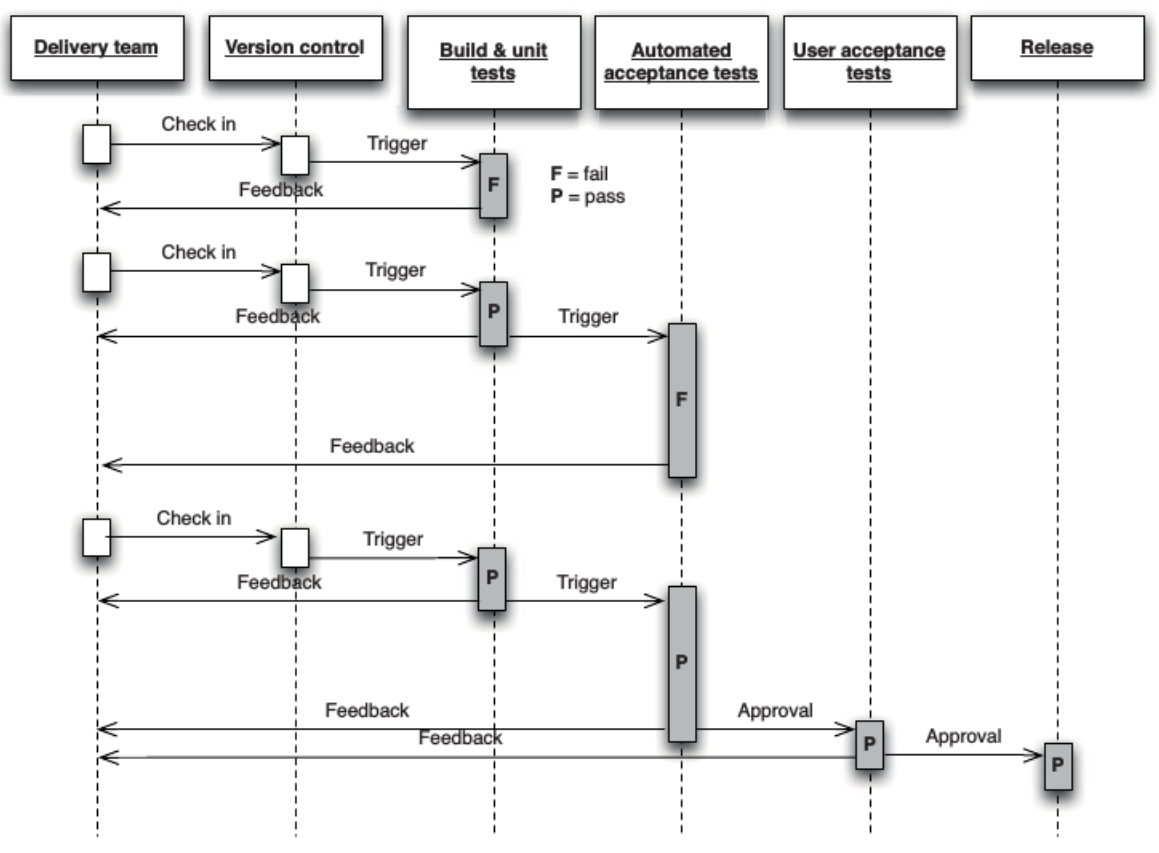
\includegraphics[width=\textwidth]{cdPipeline.png}
\end{center}

У такого подхода есть несколько важных следствий. Во-первых, вам будет крайне сложно выложить в production версии, которые не считаются пригодными для этого, конвейер просто не позволит вам этого сделать. Во-вторых, с подобной автоматизацией выкат новой версии становится быстрым, повторяемым и надёжным (всё то, чего мы так хотели в начале этой лекции). Если вы обнаруживаете, что в текущей версии появился критический баг, вы просто нажимаете пару кнопок, и происходит откат на предыдущую стабильную версию, а проблемную версию чините в оффлайне. Всё это требует автоматизации процесса тестирования, автоматического развёртывания релизов для тестирования, а также в production.

Для разных проектов набор этапов конвейера развёртывания может быть свой, однако более-менее типичные для всех этапы таковы.

\begin{center}
    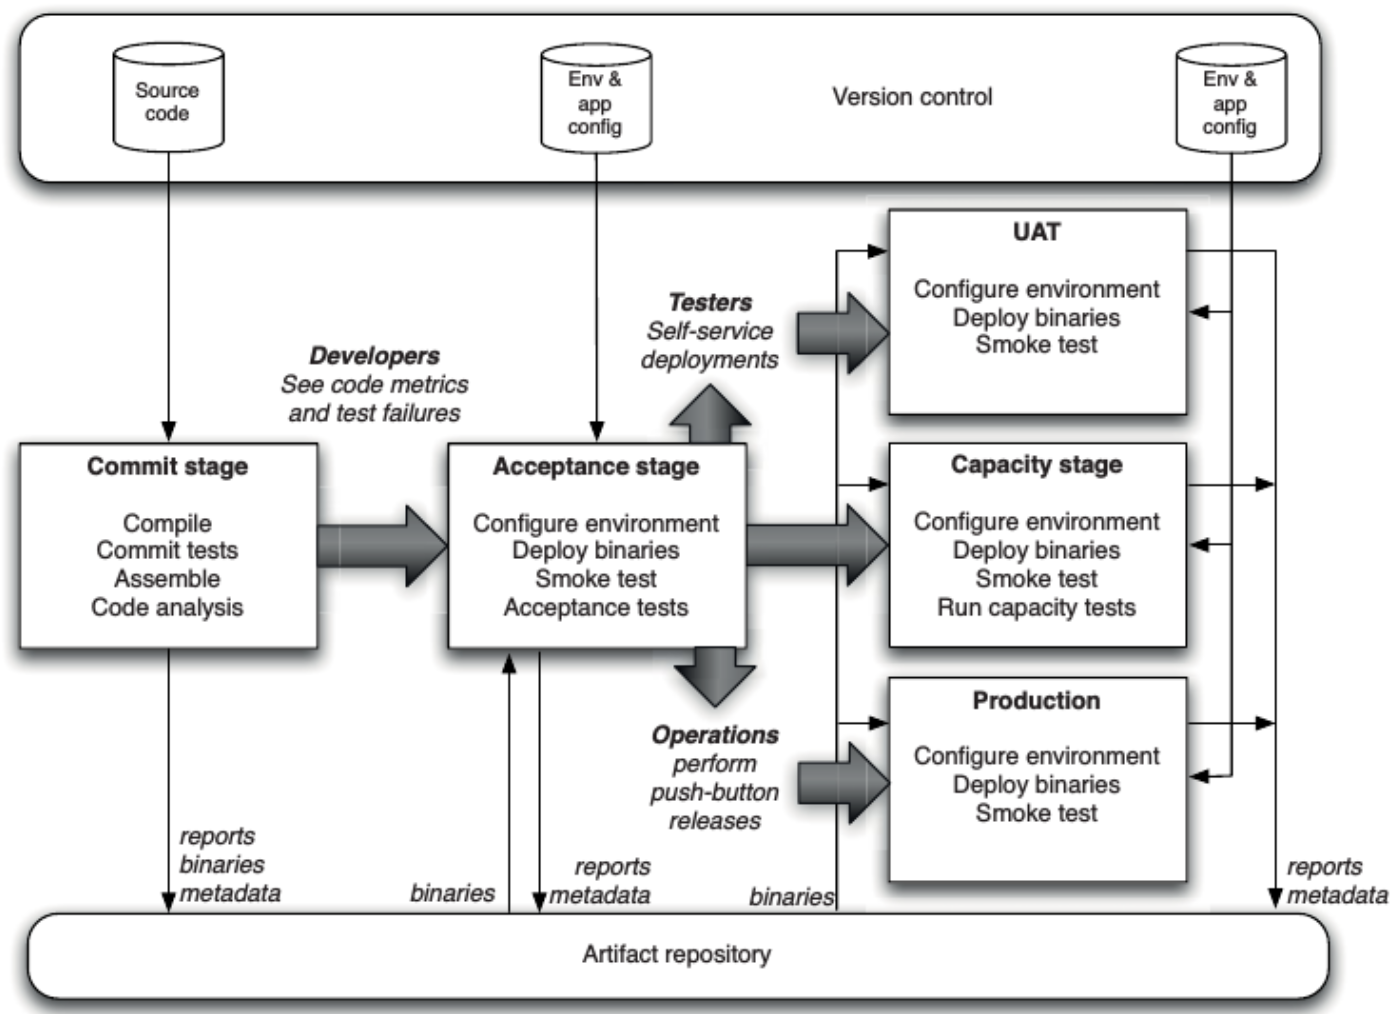
\includegraphics[width=\textwidth]{cdStages.png}
\end{center}

На \emph{стадии исходных текстов (commit stage)} мы убеждаемся, что система работает на техническом уровне: компилируется, проходит модульные автотесты, проходят проверки стиля, статический анализ кода, создаётся инсталлятор и т.п. Если на каком-то из этих шагов что-то пошло не так, все заинтересованные получают уведомление (чаще всего ответственность за результат стадии коммита лежит на команде разработки). Если всё хорошо, то создаётся исполняемый бинарник (или набор бинарников) и он сохраняется в специальном репозитории. Большинство современных CI систем берёт эту задачу на себя, представляя своим пользователям и инструментам последующих стадий удобный доступ к ним. Ну или есть специальные тулы типа Nexus\footnote{Домашняя страница Nexus, URL: \url{https://www.sonatype.com/products/sonatype-nexus-repository} (дата обращения: 21.05.2023).} или Artifactory\footnote{Домашняя страница Artifactory, URL: \url{https://jfrog.com/community/open-source/} (дата обращения: 21.05.2023).}, которые позволяют вам управлять артефактами проекта самостоятельно. Кроме бинарников выходом данной стадии являются всевозможные отчёты: результаты сборки, метрики и статистика по коду, результаты запуска модульных тестов, статического анализа и т.п.

Эта стадия должна завершаться как можно быстрее, на неё не должно уходить больше пяти минут (или десяти для очень больших проектов).

На \emph{стадии приёмочного тестирования} убеждаемся, что система работает в соответствии со своими функциональными и нефункциональными требованиями, что её поведение удовлетворяет спецификации заказчика. Эта стадия обычно запускается автоматически для каждого успешного завершения первой стадии и занимает больше времени на выполнение. Чтобы с этим бороться, современные CI-системы умеют запускать тесты параллельно на нескольких серверах или окружениях. Но для этого тесты не должны иметь общее состояние, то есть быть атомарными и автономными. С приёмочными тестами организовать это может быть непросто.

Эта стадия является вторым шагом, который обязательно должен пройти успешно кандидат в релизы. Если какие-то тесты не проходят, релиз дальше по конвейеру не идёт. На последующих стадиях, к слову, это не всегда так: например, приложение может не пройти стресс-тестирование, но всё равно быть выложено заказчику.

Далее конвейер ветвится в зависимости от окружения, в которое вы хотите развёртывать ваше ПО. Последующие стадии уже не запускаются автоматически по завершении предыдущих, а стартуют по необходимости и по команде ответственных за них специалистов.

На \emph{стадии ручного тестирования} проверяем, что система удовлетворяет пожеланиям пользователей, приносит им пользу, удобна в использовании и в ней нет никаких ошибок, которые пропустило автоматическое тестирование. Здесь обычно проводят исследовательское тестирование, тестирование на реальных пользователях и т.п.

На \emph{стадии выпуска} система поставляется разработчикам или пользователям в нужное окружение. Отдельно на этом этапе стоит подумать о возможности быстрого и эффективного отката версий. Часто оказывается удобной схема <<blue-green deployments>>, когда заводится два идентичных по инфраструктуре production-окружения, и пока одно из них доступно пользователям, на второе выкатывается и проверяется новая версия ПО. Когда есть уверенность, что новая версия работает хорошо, происходит переключение перенаправления запросов пользователя на второй вариант окружения. С базой данных при таком подходе придётся немного повозиться, да и заводить полную копию production-окружения может быть дорого (версия <<для бедных>>~--- одно окружение, в котором по аналогии запущены несколько экземпляров ПО и происходит переключение между ними при помощи настроек окружения), но если схема осуществима, она может сильно снизить число ошибок и потраченных нервов команды.

Конвейер развёртывания по-другому часто называют конвейером сборки, конвейером непрерывной интеграции или как-то ещё. Как бы его ни называли, это автоматизация процесса появления новых версий ПО из исходного кода. <<Автоматизация>> тут не означает, что в этот процесс никак не вовлечены люди, скорее то, что все сложные и критичные к ошибкам этапы выполняются автоматически, надёжно и повторяемо. А человеческое участие сводится к управлению этими процессами. Тестировщики могут в один клик развернуть нужную версию в нужном тестовом окружении. Системные администраторы в один клик могут развернуть нужную версию ПО на production-серверах. Разработчики видят, какие версии находятся на каких этапах конвейера, и в чём состоят проблемы, если они возникают. Менеджеры могут автоматизировать вычисление интересующих их метрик (например, длительность всего цикла конвейера, пропускная способность, качество ПО и т.п.). Все получают доступ к информации и действиям, которые им необходимо выполнить, а также прозрачность всего процесса.

\subsection{Полезные практики}

\subsubsection{Собираем бинарники только один раз}

Для удобства будем под бинарниками понимать любой выполняемый код, включая интерпретируемые скрипты.

Многие системы сборки используют в качестве входа на любом шаге исходный код из системы контроля версий. Это приводит к тому, что происходит многократная сборка кода в разных контекстах: после коммита, на стадии приёмочного тестирования, для каждого из целевых окружений и т.п. Подобную ситуацию вполне можно считать антипаттерном, который нарушает два важных принципа. Во-первых, конвейер сборки должен быть эффективным, чтобы команда могла получать обратную связь как можно быстрее. А сборка, особенно в крупных проектах и на языках типа С++, может занимать довольно много времени. Во-вторых, каждый раз при сборке вы вносите риск получить немного другой бинарник: у вас может быть немного отличающаяся версия компилятора или его конфигурация, другая версия третьесторонней библиотеки и т.п. А это всё потенциальные сложнообнаружимые ошибки. Уж не говоря о том, что за время между стадиями исходный код в репозитории может поменяться.

Итого, бинарник, который выкладывается в production, должен быть в точности тот же, который создавался на стадии коммита и проходил через все стадии тестирования. Чтобы обеспечить это, многие CI-системы сохраняют все создаваемые бинарники и проверяют их хеш-коды от стадии к стадии конвейера, что это именно те бинарники, которые нужны. Но бэкапить без особой нужды бинарники вряд ли имеет смысл: если что, их всегда можно собрать заново, зная нужную версию кода.

\subsubsection{Один и тот же процесс развёртывания для разных окружений}

Крайне важно использовать один и тот же процесс для развёртывания всех окружений, начиная от локальной машины разработчика и заканчивая production-вариантом. Это поможет лучше протестировать процесс развёртывания, и тем самым снизить риски выкладывания боевой версии заказчику.

Каждое окружение имеет свои особенности. Как минимум отличаются IP-адреса целевых серверов, однако часто также это разные версии ОС, настроек вспомогательных библиотек и фреймворков, адреса и имена баз данных и внешних сервисов и другая конфигурационная информация. И тут нужно держать себя в руках и не создавать под каждый вариант окружения свой скрипт установки. В таких случаях имеет смысл выделить изменяющиеся компоненты в конфигурацию скрипта и хранить такие наборы настроек отдельно, например, в разных файлах. Разумеется, эти файлы настроек скрипта должны храниться в системе контроля версий и быть доступны по IP-адресу, названию окружения или чему-то ещё, передаваемому в переменных окружения скрипту развёртывания. Эта практика~--- ещё одно применения правила <<держите то, что меняется и то, что не меняется, отдельно друг от друга>>.

В итоге у вас будет один скрипт и набор конфигурационных файлов к нему, меняющих его поведение. Так что если при развёртывании приложения в какое-то окружение что-то пошло не так, то это по одной из трёх причин:

\begin{itemize}
    \item ошибка в настройках конфигурационного файла, соответствующего данному окружению;
    \item проблема в инфраструктуре или в одном из сервисов, от которых зависит приложение;
    \item ошибка в настройках окружения.
\end{itemize}

\subsubsection{Запуск smoke test’ов после развёртывания}

Когда вы выкладываете приложение, вам обязательно нужен автоматический скрипт, который проверит, что приложение запустилось и работает как надо. Это может быть что-то очень простое типа запуска приложения и проверки, что открывается главная страница с ожидаемым содержимым. Этот тест также должен проверять, что также работают все сервисы, от которых зависит ваше приложение: базы данных, шина сообщений, внешние сервисы и т.п.

Этот тест по важности не уступает модульным тестам: он даёт вам уверенность, что приложение действительно запустилось. Если же приложение не запустилось, то этот тест должен проводить базовую диагностику и выдавать вам информацию по её итогам. По крайней мере, что именно не заработало.

\subsubsection{Развёртывание в копии production окружения}

Ещё одна проблема, с которой сталкиваются во многих проектах~--- окружения, в которых ведётся разработка и тестирование ПО, совсем не похожи на окружение, в котором ему придётся работать у заказчика. Никакой уверенности в том, что приложение хорошо заработает в production’е, такое положение дел, разумеется, не даёт.

В идеале, если ваше production-окружение простое или у вас достаточный бюджет, хорошо бы иметь точную копию production-окружения у себя локально для запуска автоматических и ручных тестов. Поддержка такой идентичности потребует аккуратности в конфигурационном управлении. Нужно убедиться, что одинаковы конфигурации инфраструктуры (сетевая топология, настройки сетевых соединений, фаерволов и т.д.), операционных систем (включая наборы патчей, установленных обновлений и пр.), стека приложений, что данные приложений в корректном состоянии (например, развёрнута правильная версия базы данных) и т.п.

\subsection{Создание конвейера развёртывания}

Начинаете ли вы новый проект или пытаетесь внедрить автоматизированный конвейер в уже существующий проект, почти всегда имеет смысл двигаться инкрементально. Рассмотрим самые типовые шаги этого процесса.

\subsubsection{Проектирование основных этапов и создание рабочего скелета}

Как уже говорилось ранее, первый шаг~--- определиться с шагами, которые проходит ваше ПО от коммита до релиза. Если проект уже запущен и работает, на это потребуется максимум полчаса, надо всего лишь пойти и поговорить с теми, кто вовлечён в этот процесс, и аккуратно всё записать. Если проект новый, то этот конвейер надо придумать. Один из вариант~--- посмотреть на другие похожие проекты внутри компании и сделать похожим образом. Или, если это не вариант, можно начать с самого минимума: с фазы коммита, включающей сборку приложения и прогон основных метрик и модульных тестов, фазы приёмочного тестирования и фазы развёртывания приложения в production-like окружение для демонстраций.

Как только определите свой процесс, можно начать моделировать его в тулах для CI. Если тул явно не даёт нарисовать flow, можно просто завести там несколько подпроектов и расставить между ними зависимости так, чтобы они выполнялись друг за другом. Если проект ещё совсем только начинается, некоторые из этих этапов могут дёргать уже существующие скрипты либо просто быть заглушками. Ваша задача~--- построить скелет процесса, где каждый этап выполняет самый минимальный объём работы, необходимый на этом шаге. Например, первый шаг~--- фаза коммита. Если ещё нет никакого кода и тестов, создайте самое минимальное приложение <<Hello world>> и один модульный тест, который делает assertTrue(true). На фазе развёртывания этот бинарник будет копироваться в нужную папку на сервере, а на фазе приёмочного тестирования вы будете проверять доступность этого приложения, запускать его и убеждаться, что оно выдаёт текст <<Hello world>>.

В новом проекте вся эта работа по идее должна быть выполнена до того, как начнётся собственно разработка~--- так называемая <<итерация 0>>, если используется итеративная модель разработки.

\subsubsection{Автоматизирование сборки и развёртывания}

Первая стадия конвейера почти всегда~--- автоматизированная сборка ПО из исходников. Для интерпретируемых языков никакой компиляции как таковой может и не происходить, но всё равно должен быть подготовлен самодостаточный набор исполняемых файлов для копирования на другие компьютеры и запуска там без каких-либо зависимостей от инструментов разработчика. Такой процесс сборки должен проводиться каждый раз, как кто-то выкладывает что-то новое в систему контроля версий. Раньше это делалось регулярным опросом CI-тула системы контроля версий, сейчас же более распространены хуки (hooks)~--- скрипты, позволяющие системе контроля версий дёргать внешние сервисы по заданным событиям. Для небольшого проекта получаемые сборки могут выкладываться на этом же CI-сервере, для более крупных проектов могут понадобиться отдельные сервера, максимально похожие по конфигурации на целевые окружения. Чуть более сложная задача~--- развёртывание набора приложений по разным серверам одновременно, но и она решается при должном уровне автоматизации. И не забываем про простой smoke-тест, проверяющий, что приложение установилось корректно и работает.

\subsubsection{Автоматизирование модульных тестов и анализа кода}

Далее надо довести до ума фазу коммита~--- реализовать запуск модульных тестов, анализа стиля и структуры кода, выбор приёмочных и интеграционных тестов для запуска после каждого коммита. Но нужно не увлекаться и помнить, что эта фаза должна завершаться как можно быстрее: не дольше нескольких минут для средних по размеру проектов. Так что в этих тестах не должны использоваться файловая система, базы данных и т.п. На этой стадии хорошо собирать разного рода метрики: покрытие кода тестами, сложность, сопряжение и связность модулей и т.п. С ростом приложения модульных тестов будет становиться всё больше и больше, и их стоит начать разбивать на test suite’ы и запускать параллельно на одной или нескольких машинах.

\subsubsection{Автоматизирование приёмочных тестов}

Приёмочные тесты делятся на две группы: функциональные и нефункциональные. С первыми всё более-менее понятно, а вот нефункциональные тесты по-хорошему надо начинать создавать в самом начале проекта, чтобы убедиться, насколько система удовлетворяет нефункциональным требованиям: масштабируемости, отказоустойчивости, нагруженности и т.п. Хорошие приёмочные тесты позволят вам находить ошибки типа гонок и дедлоков, которые может быть сложно воспроизвести локально на компьютерах разработчиков. Так что система, запускающая приёмочные тесты, должна собирать достаточно информации о работе тестов и системы: как минимум подробные логи, а то и снимки экранов. При отладке потом всё это очень пригодится.

\subsubsection{Эволюционирование конвейера}

С ростом проекта конвейер становится больше и сложнее, его развитие происходит чаще всего в двух направлениях: поддержка компонент и ветвлений. В случаях, когда приложение начинает состоять из набора крупных компонент, бывает оправданным заводить отдельный конвейер для каждой компоненты, а потом по завершении каждого их них собирать приложение и проверять его уже как единое целое.

При построении и дальнейшей эволюции конвейера надо понимать, что не нужно пытаться сделать всё и сразу. Это долго, дорого и почти всегда не особо приоритетно. Если часть работы выполняется вручную, оставьте для неё заглушку, зафиксировав, сколько времени уходит на этот этап. И когда именно этот этап станет узким местом конвейера, тогда надо браться за его автоматизацию. Говоря об узких местах, помимо сбора метрик о приложении полезной практикой является сбор метрик о работе самого конвейера: сколько времени уходит на каждый его этап, сколько раз вообще запускался конвейер, сколько из этих запусков успешно прошло все шаги и т.п.

\section{Модель зрелости процесса управления релизами}

Ну и под конец поговорим о модели, которая позволяет оценить зрелость описанных практик в масштабе проекта или организации. Цели всех этих практик таковы:

\begin{itemize}
    \item снизить длительность цикла выпуска версий, что влечёт за собой более быструю поставку новой функциональности заказчикам и увеличение прибыли;
    \item снизить количество дефектов, чтобы тратить меньше времени и денег на поддержку и исправление ошибок;
    \item повысить предсказуемость процесса выхода новых версий ПО для более эффективного планирования работ;
    \item иметь возможность оценивать и эффективно управлять рисками, связанными с выходом новых версий;
    \item общее снижение затрат ввиду лучшего управления рисками и меньшего количества проблем, связанных с выпуском версий.
\end{itemize}

В достижении этих целей может помочь модель на рисунке ниже. Для начала можно просто посмотреть на организацию процессов в проектах и оценить каждую практику по предлагаемой шкале. Отдельные проекты могут быть на разных уровнях в каждой категории. Затем надо оценить, какие практики тормозят весь процесс больше всего, сколько будет стоить улучшение этих практик, сколько вы сможете получить или сэкономить после их внедрения. 

\begin{center}
    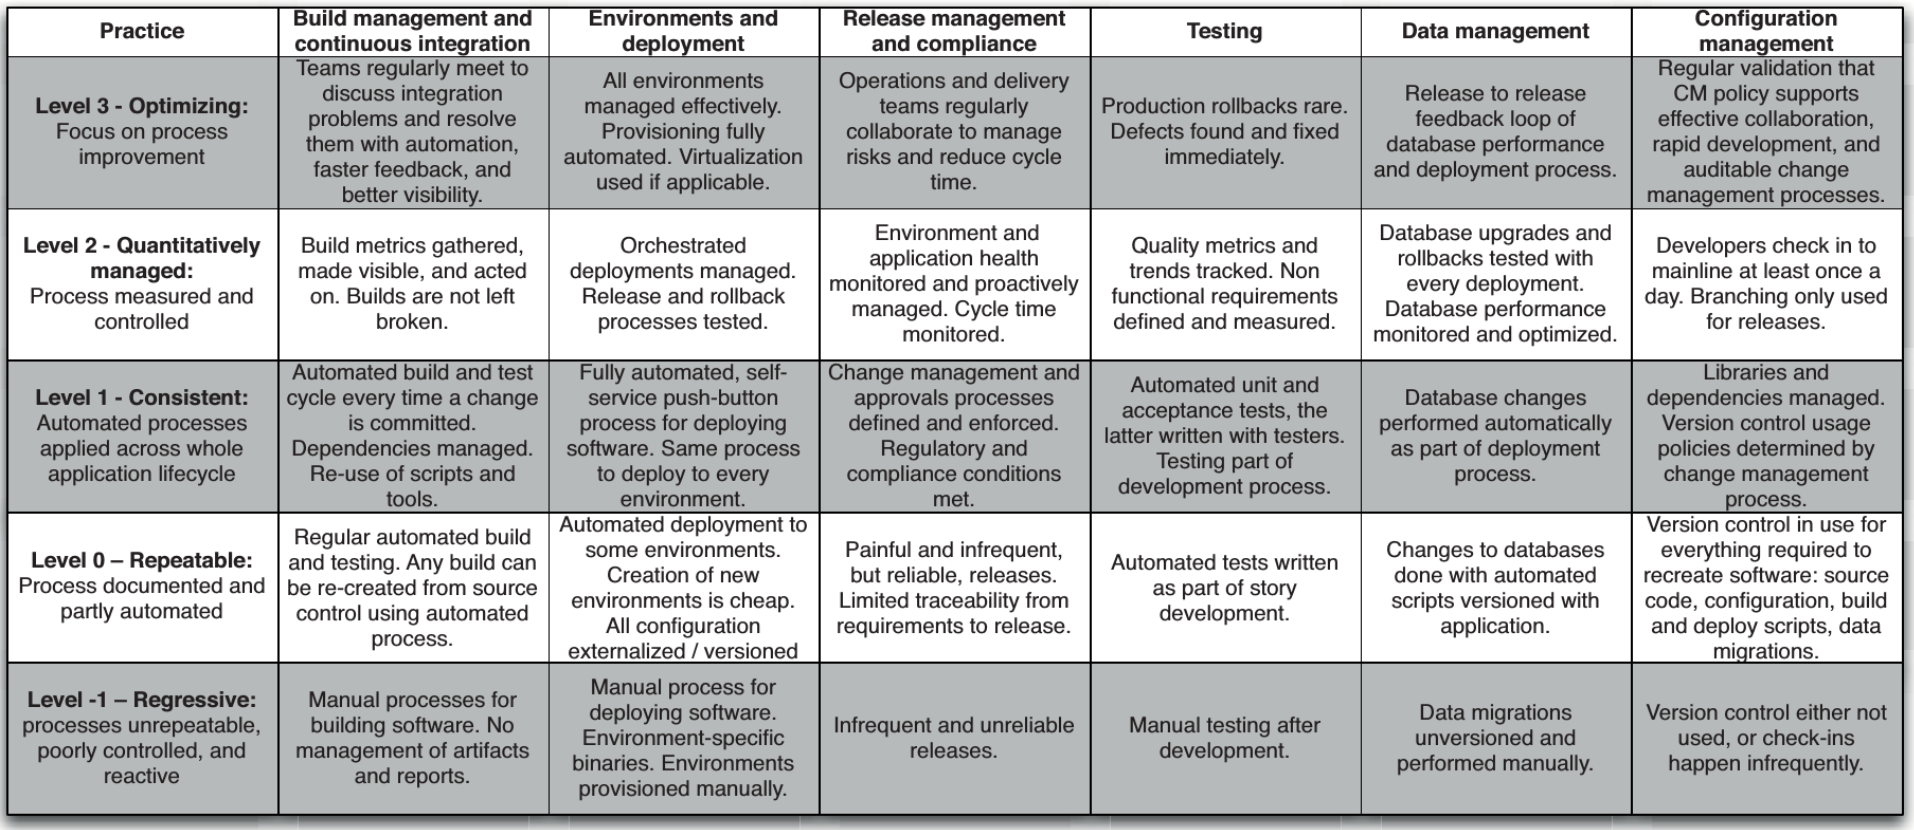
\includegraphics[width=\textwidth]{cdMaturityModel.png}
\end{center}

Дальше приоритизация и исполнение. Как уже говорилось ранее, внедрение какой-либо практики имеет смысл делать инкрементально, и начать стоит с proof-of-concept внедрения в проекте, где с этой практикой хуже всего. Это позволит получить самый большой позитивный прирост и, возможно, получить дополнительную поддержку в распространении этой практики на другие проекты или команды. Не забываем про коммуникации в процессе внедрения практик и ретроспективы по завершению намеченных этапов. Это позволит отслеживать свой прогресс и не отклоняться от выбранного направления.

\end{document}